% Appendix Template

\newcommand{\major}{4}
\newcommand{\minor}{2}

\newcommand{\undPrefix}{\major_\minor}
\newcommand{\dotPrefix}{\major.\minor}
\newcommand{\scoPrefix}{\major-\minor}
\newcommand{\filePrefix}{\undPrefix/rff}

\chapter{Results of experiment \dotPrefix} % Main appendix title


\label{Appendix\scoPrefix} % Change X to a consecutive letter; for referencing this appendix elsewhere, use \ref{AppendixX}

These experiments are discussed \hyperref[disc:h4]{here}


%%%%%%%%%%%%%%%%%%%%%%%%%%%%%%%%%%%%%%%%%%%%%%
%%%%%%%%%%%%%%%%%%%%%%%%%%%%%%%%%%%%%%%%%%%%%%
%%%%%%%%%%%%%%%%%%%%%%%%%%%%%%%%%%%%%%%%%%%%%%
%% Empieza lo nuevo
%%%%%%%%%%%%%%%%%%%%%%%%%%%%%%%%%%%%%%%%%%%%%%
%%%%%%%%%%%%%%%%%%%%%%%%%%%%%%%%%%%%%%%%%%%%%%
%%%%%%%%%%%%%%%%%%%%%%%%%%%%%%%%%%%%%%%%%%%%%%

\begin{figure}[H]
  \centering
  \renewcommand{\filePrefix}{\undPrefix/rff}
  \begin{subfigure}[t]{0.5\linewidth}
    \centering\captionsetup{width=.8\linewidth}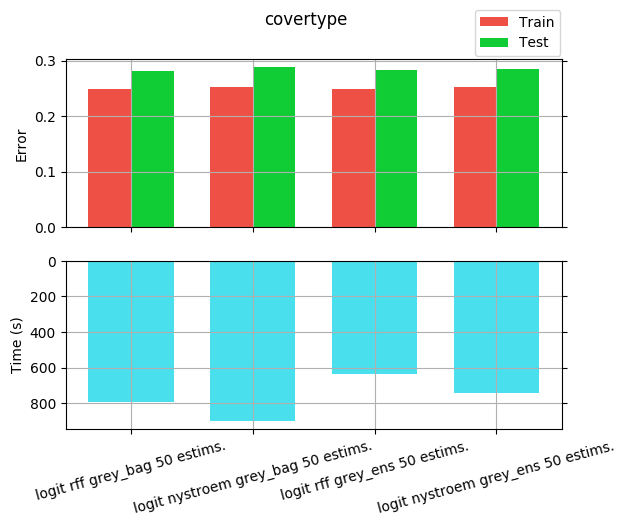
\includegraphics[width=\imgscale\linewidth]{Figures/\filePrefix/covertype}
    % \caption{Exp. 4.2 with Covertype. Random Forest outperforms Ensembles of Decision Tree with RFF.}
    \label{fig:\undPrefix_covertype}
  \end{subfigure}%
  \renewcommand{\filePrefix}{\undPrefix/nys}%
  \begin{subfigure}[t]{0.5\linewidth}
    \centering\captionsetup{width=.8\linewidth}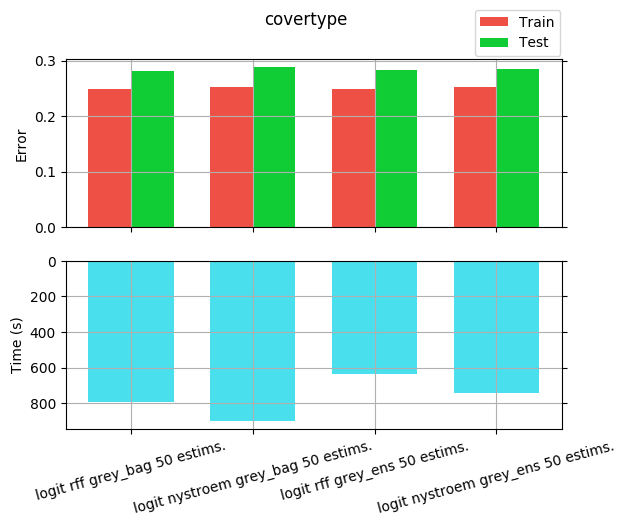
\includegraphics[width=\imgscale\linewidth]{Figures/\filePrefix/covertype}
    % \caption{Exp. 4.2 with Covertype. Random Forest outperforms Ensembles of Decision Tree with \Nys.}
    \label{fig:\undPrefix_covertype}
  \end{subfigure}%
  \caption*{Exp. 4.2 with Covertype. Random Forest outperforms Ensembles of
  Decision Tree with RFF (left) and \Nys\ (right).}
\end{figure}


\begin{figure}[H]
  \centering
  \renewcommand{\filePrefix}{\undPrefix/rff}
  \begin{subfigure}[t]{0.5\linewidth}
    \centering\captionsetup{width=.8\linewidth}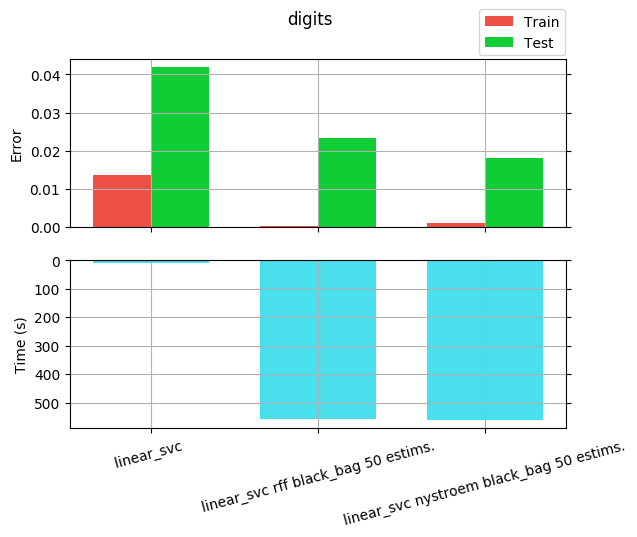
\includegraphics[width=\imgscale\linewidth]{Figures/\filePrefix/digits}
    % \caption{Exp. 4.2 with Digits. Random Forest outperforms Ensembles of Decision Tree with RFF.}
    \label{fig:\undPrefix_digits}
  \end{subfigure}%
  \renewcommand{\filePrefix}{\undPrefix/nys}%
  \begin{subfigure}[t]{0.5\linewidth}
    \centering\captionsetup{width=.8\linewidth}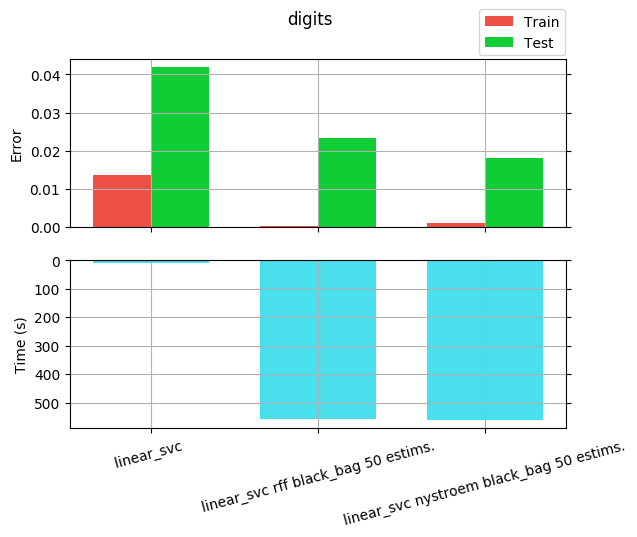
\includegraphics[width=\imgscale\linewidth]{Figures/\filePrefix/digits}
    % \caption{Exp. 4.2 with Digits. Random Forest outperforms Ensembles of Decision Tree with \Nys.}
    \label{fig:\undPrefix_digits}
  \end{subfigure}
  \caption*{Exp. 4.2 with Digits. Random Forest outperforms Ensembles of Decision Tree with RFF (left) and \Nys\ (right).}
\end{figure}


\begin{figure}[H]
  \centering
  \renewcommand{\filePrefix}{\undPrefix/rff}
  \begin{subfigure}[t]{0.5\linewidth}
    \centering\captionsetup{width=.8\linewidth}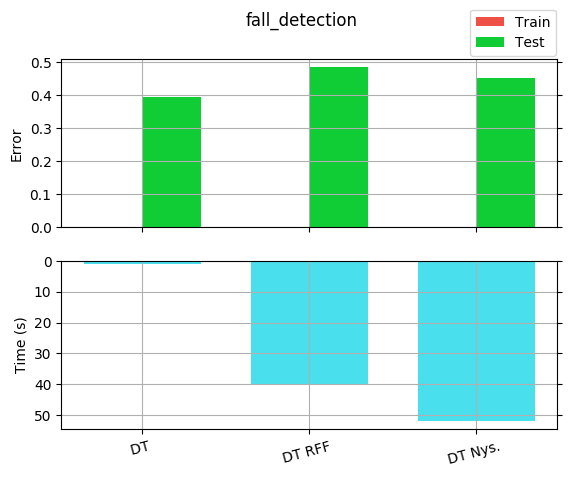
\includegraphics[width=\imgscale\linewidth]{Figures/\filePrefix/fall_detection}
    % \caption{Exp. 4.2 with Fall Detection. Random Forest outperforms Ensembles of Decision Tree with RFF.}
    \label{fig:\undPrefix_fall_detection}
  \end{subfigure}%
  \renewcommand{\filePrefix}{\undPrefix/nys}%
  \begin{subfigure}[t]{0.5\linewidth}
    \centering\captionsetup{width=.8\linewidth}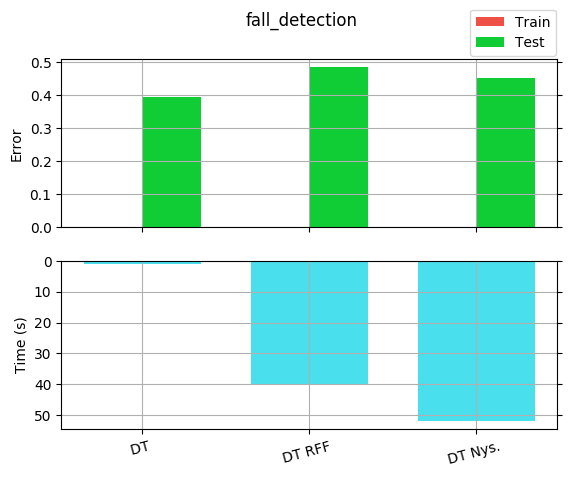
\includegraphics[width=\imgscale\linewidth]{Figures/\filePrefix/fall_detection}
    % \caption{Exp. 4.2 with Fall Detection. Random Forest outperforms Ensembles of Decision Tree with \Nys.}
    \label{fig:\undPrefix_fall_detection}
  \end{subfigure}%
  \caption*{Exp. 4.2 with Fall Detection. Random Forest outperforms Ensembles of Decision Tree with RFF (left) and \Nys\ (right).}
\end{figure}


\begin{figure}[H]
  \centering
  \renewcommand{\filePrefix}{\undPrefix/rff}
  \begin{subfigure}[t]{0.5\linewidth}
    \centering\captionsetup{width=.8\linewidth}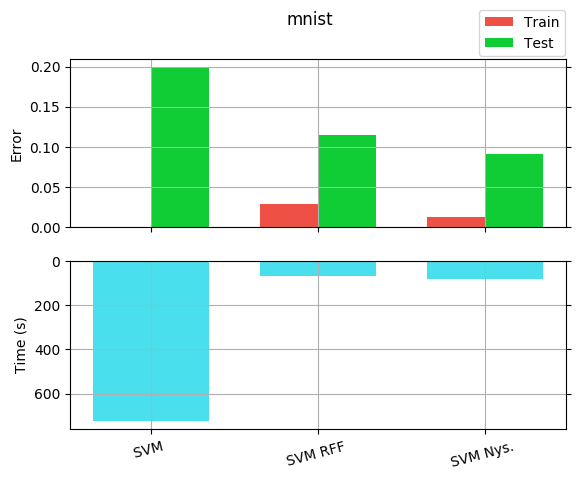
\includegraphics[width=\imgscale\linewidth]{Figures/\filePrefix/mnist}
    % \caption{Exp. 4.2 with MNIST. Random Forest outperforms Ensembles of Decision Tree with RFF.}
    \label{fig:\undPrefix_mnist}
  \end{subfigure}%
  \renewcommand{\filePrefix}{\undPrefix/nys}%
  \begin{subfigure}[t]{0.5\linewidth}
    \centering\captionsetup{width=.8\linewidth}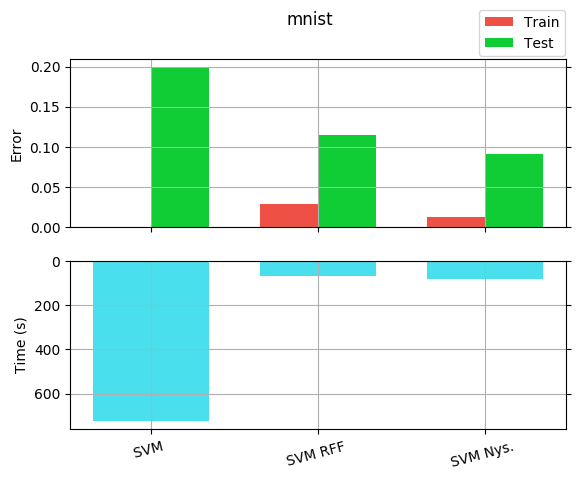
\includegraphics[width=\imgscale\linewidth]{Figures/\filePrefix/mnist}
    % \caption{Exp. 4.2 with MNIST. Random Forest outperforms Ensembles of Decision Tree with \Nys.}
    \label{fig:\undPrefix_mnist}
  \end{subfigure}
  \caption*{Exp. 4.2 with MNIST. Random Forest outperforms Ensembles of Decision Tree with RFF (left) and \Nys\ (right).}
\end{figure}


\begin{figure}[H]
  \centering
  \renewcommand{\filePrefix}{\undPrefix/rff}
  \begin{subfigure}[t]{0.5\linewidth}
    \centering\captionsetup{width=.8\linewidth}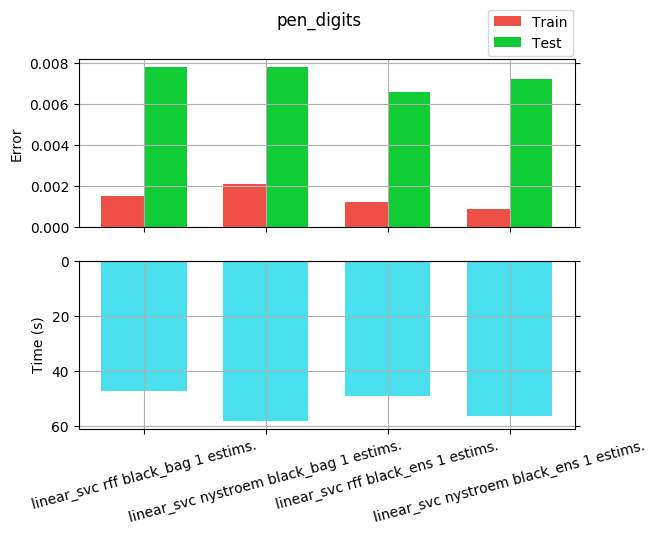
\includegraphics[width=\imgscale\linewidth]{Figures/\filePrefix/pen_digits}
    % \caption{Exp. 4.2 with Pen Digits. Random Forest outperforms Ensembles of Decision Tree with RFF.}
    \label{fig:\undPrefix_pen_digits}
  \end{subfigure}%
  \renewcommand{\filePrefix}{\undPrefix/nys}%
  \begin{subfigure}[t]{0.5\linewidth}
    \centering\captionsetup{width=.8\linewidth}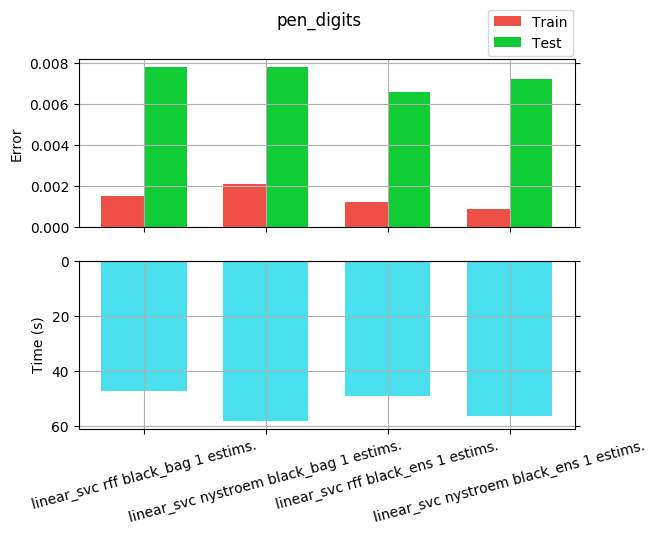
\includegraphics[width=\imgscale\linewidth]{Figures/\filePrefix/pen_digits}
    % \caption{Exp. 4.2 with Pen Digits. Random Forest outperforms Ensembles of Decision Tree with \Nys.}
    \label{fig:\undPrefix_pen_digits}
  \end{subfigure}%
  \caption*{Exp. 4.2 with Pen Digits. Random Forest outperforms Ensembles of Decision Tree with RFF (left) and \Nys\ (right).}
\end{figure}


\begin{figure}[H]
  \centering
  \renewcommand{\filePrefix}{\undPrefix/rff}
  \begin{subfigure}[t]{0.5\linewidth}
    \centering\captionsetup{width=.8\linewidth}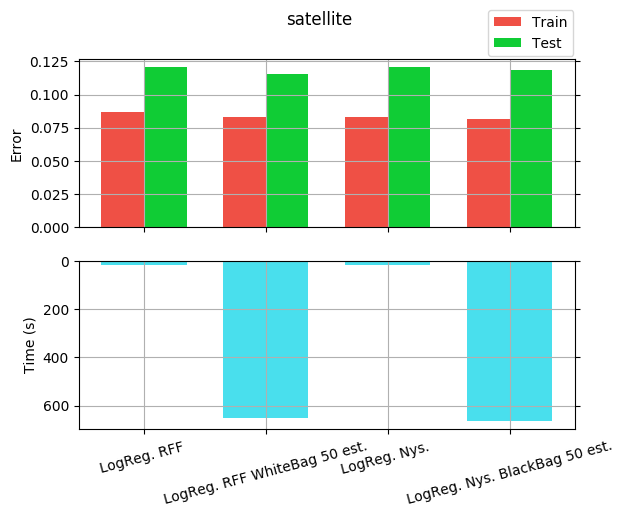
\includegraphics[width=\imgscale\linewidth]{Figures/\filePrefix/satellite}
    % \caption{Exp. 4.2 with Satellite. Random Forest outperforms Ensembles of Decision Tree with RFF.}
    \label{fig:\undPrefix_satellite}
  \end{subfigure}%
  \renewcommand{\filePrefix}{\undPrefix/nys}%
  \begin{subfigure}[t]{0.5\linewidth}
    \centering\captionsetup{width=.8\linewidth}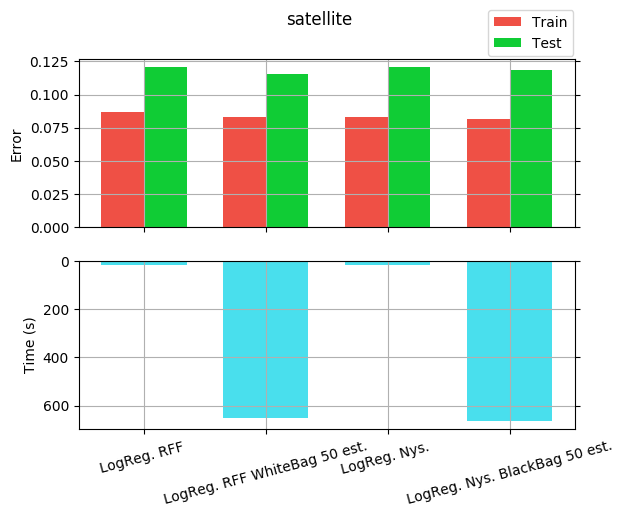
\includegraphics[width=\imgscale\linewidth]{Figures/\filePrefix/satellite}
    % \caption{Exp. 4.2 with Satellite. Random Forest outperforms Ensembles of Decision Tree with \Nys.}
    \label{fig:\undPrefix_satellite}
  \end{subfigure}
  \caption*{Exp. 4.2 with Satellite. Random Forest outperforms Ensembles of Decision Tree with RFF (left) and \Nys\ (right).}
\end{figure}


\begin{figure}[H]
  \centering
  \renewcommand{\filePrefix}{\undPrefix/rff}
  \begin{subfigure}[t]{0.5\linewidth}
    \centering\captionsetup{width=.8\linewidth}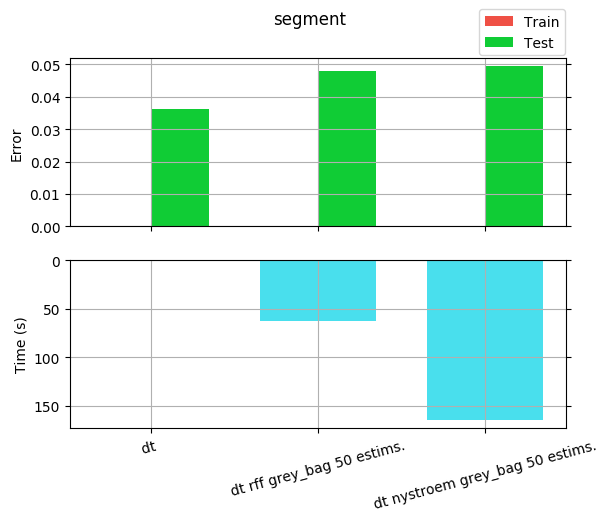
\includegraphics[width=\imgscale\linewidth]{Figures/\filePrefix/segment}
    % \caption{Exp. 4.2 with Segment. Random Forest outperforms Ensembles of Decision Tree with RFF.}
    \label{fig:\undPrefix_segment}
  \end{subfigure}%
  \renewcommand{\filePrefix}{\undPrefix/nys}%
  \begin{subfigure}[t]{0.5\linewidth}
    \centering\captionsetup{width=.8\linewidth}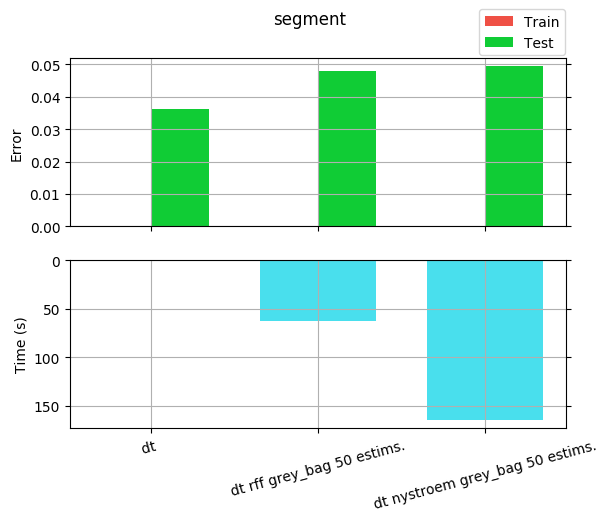
\includegraphics[width=\imgscale\linewidth]{Figures/\filePrefix/segment}
    % \caption{Exp. 4.2 with Segment. Random Forest outperforms Ensembles of Decision Tree with \Nys.}
    \label{fig:\undPrefix_segment}
  \end{subfigure}%
  \caption*{Exp. 4.2 with Segment. Random Forest outperforms Ensembles of Decision Tree with RFF (left) and \Nys\ (right).}
\end{figure}


\begin{figure}[H]
  \centering
  \renewcommand{\filePrefix}{\undPrefix/rff}
  \begin{subfigure}[t]{0.5\linewidth}
    \centering\captionsetup{width=.8\linewidth}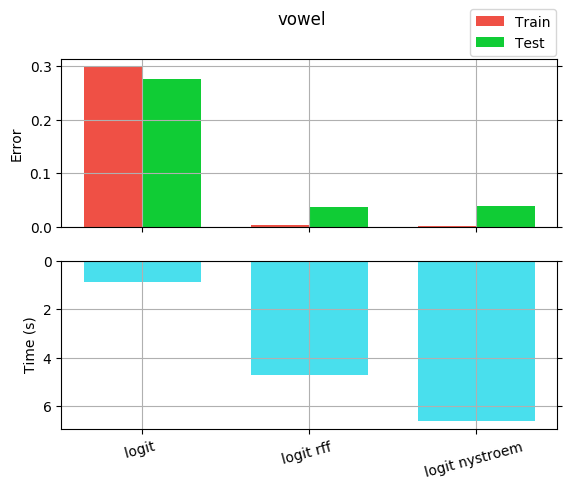
\includegraphics[width=\imgscale\linewidth]{Figures/\filePrefix/vowel}
    % \caption{Exp. 4.2 with Vowel. Random Forest outperforms Ensembles of Decision Tree with RFF.}
    \label{fig:\undPrefix_vowel}
  \end{subfigure}%
  \renewcommand{\filePrefix}{\undPrefix/nys}%
  \begin{subfigure}[t]{0.5\linewidth}
    \centering\captionsetup{width=.8\linewidth}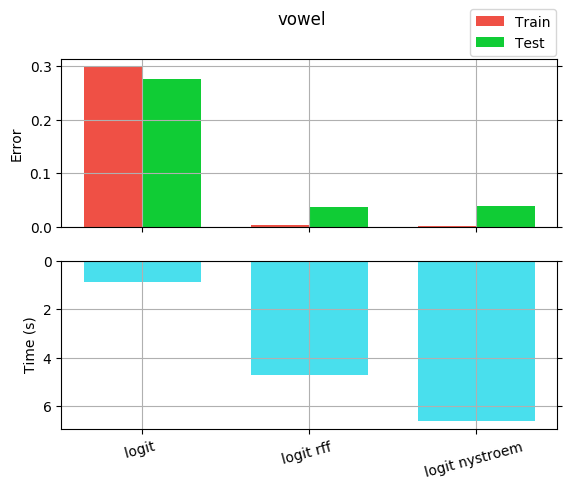
\includegraphics[width=\imgscale\linewidth]{Figures/\filePrefix/vowel}
    % \caption{Exp. 4.2 with Vowel. Random Forest outperforms Ensembles of Decision Tree with \Nys.}
    \label{fig:\undPrefix_vowel}
  \end{subfigure}
  \caption*{Exp. 4.2 with Vowel. Random Forest outperforms Ensembles of Decision Tree with RFF (left) and \Nys\ (right).}
\end{figure}


\begin{figure}[H]
  \centering
  \renewcommand{\filePrefix}{\undPrefix/rff}
  \begin{subfigure}[t]{0.5\linewidth}
    \centering\captionsetup{width=.8\linewidth}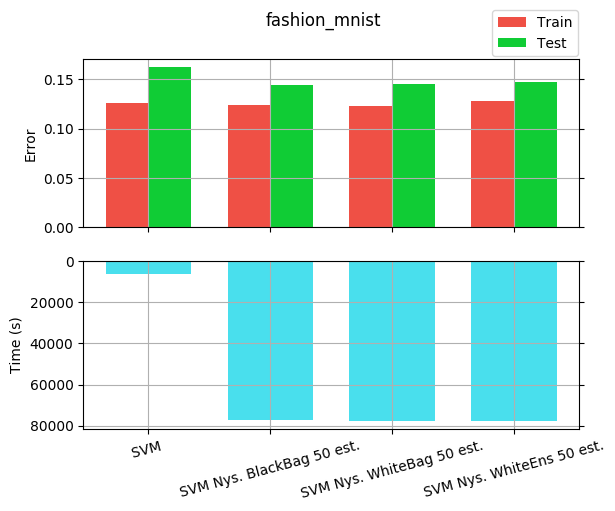
\includegraphics[width=\imgscale\linewidth]{Figures/\filePrefix/fashion_mnist}
    % \caption{Exp. 4.2 with Fashion MNIST. Random Forest outperforms Ensembles of Decision Tree with RFF.}
    \label{fig:\undPrefix_vowel}
  \end{subfigure}%
  \renewcommand{\filePrefix}{\undPrefix/nys}%
  \begin{subfigure}[t]{0.5\linewidth}
    \centering\captionsetup{width=.8\linewidth}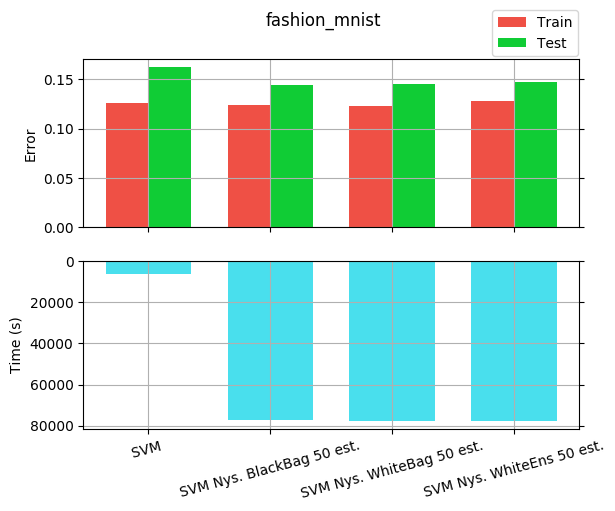
\includegraphics[width=\imgscale\linewidth]{Figures/\filePrefix/fashion_mnist}
    % \caption{Exp. 4.2 with Fashion MNIST. Random Forest outperforms Ensembles of Decision Tree with \Nys.}
    \label{fig:\undPrefix_vowel}
  \end{subfigure}
  \caption*{Exp. 4.2 with Fashion MNIST. Random Forest outperforms Ensembles of Decision Tree with RFF (left) and \Nys\ (right).}
\end{figure}


%%%%%%%%%%%%%%%%%%%%%%%%%%%%%%%%%%%%%%%%%%%%%%
%%%%%%%%%%%%%%%%%%%%%%%%%%%%%%%%%%%%%%%%%%%%%%
%%%%%%%%%%%%%%%%%%%%%%%%%%%%%%%%%%%%%%%%%%%%%%
%% Termina lo nuevo
%%%%%%%%%%%%%%%%%%%%%%%%%%%%%%%%%%%%%%%%%%%%%%
%%%%%%%%%%%%%%%%%%%%%%%%%%%%%%%%%%%%%%%%%%%%%%
%%%%%%%%%%%%%%%%%%%%%%%%%%%%%%%%%%%%%%%%%%%%%%


% \begin{figure}[H]
%   \centering
%   \begin{subfigure}[t]{0.5\linewidth}
%     \centering\captionsetup{width=.8\linewidth}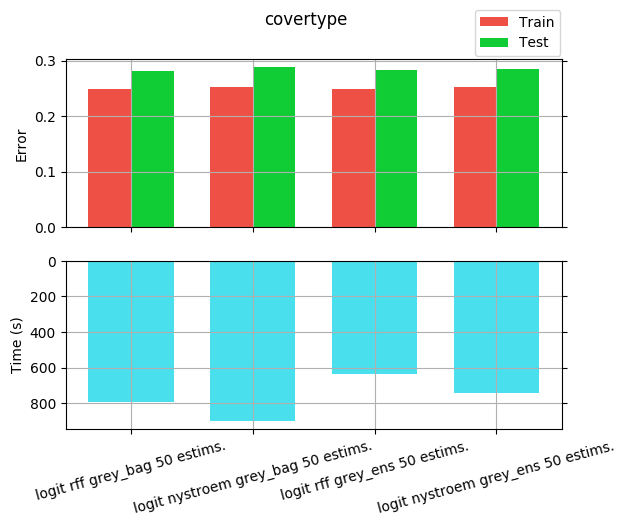
\includegraphics[width=\imgscale\linewidth]{Figures/\filePrefix/covertype}
%     \caption{Exp. 4.2 with Covertype. Random Forest outperforms Ensembles of Decision Tree with RFF.}
%     \label{fig:\undPrefix_covertype}
%   \end{subfigure}%
%   \begin{subfigure}[t]{0.5\linewidth}
%     \centering\captionsetup{width=.8\linewidth}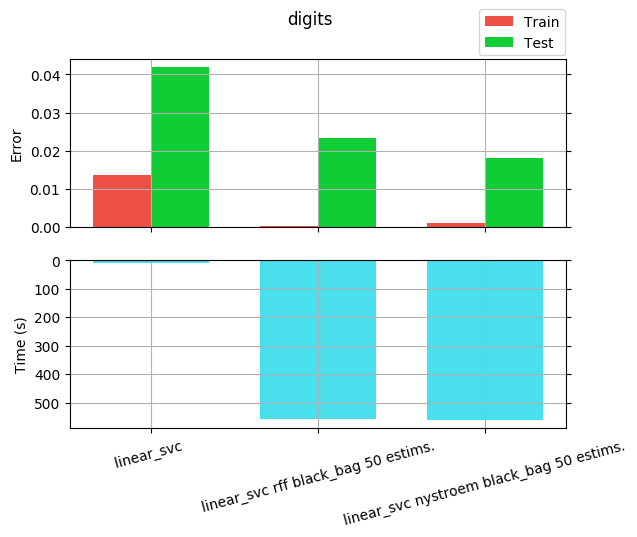
\includegraphics[width=\imgscale\linewidth]{Figures/\filePrefix/digits}
%     \caption{Exp. 4.2 with Digits. Random Forest outperforms Ensembles of Decision Tree with RFF.}
%     \label{fig:\undPrefix_digits}
%   \end{subfigure}
% \end{figure}
%
%
% \begin{figure}[H]
%   \centering
%   \begin{subfigure}[t]{0.5\linewidth}
%     \centering\captionsetup{width=.8\linewidth}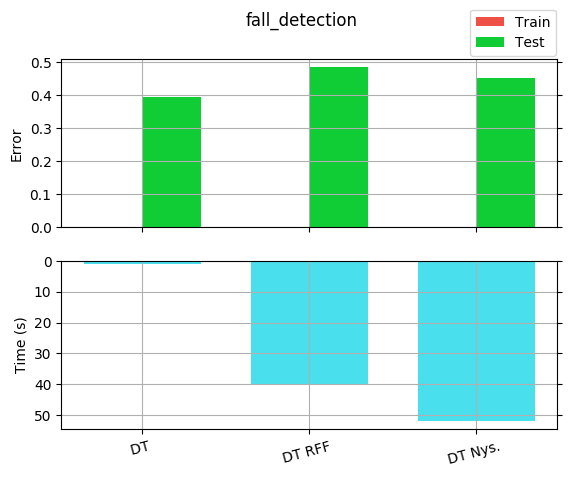
\includegraphics[width=\imgscale\linewidth]{Figures/\filePrefix/fall_detection}
%     \caption{Exp. 4.2 with Fall Detection. Random Forest outperforms Ensembles of Decision Tree with RFF.}
%     \label{fig:\undPrefix_fall_detection}
%   \end{subfigure}%
%   \begin{subfigure}[t]{0.5\linewidth}
%     \centering\captionsetup{width=.8\linewidth}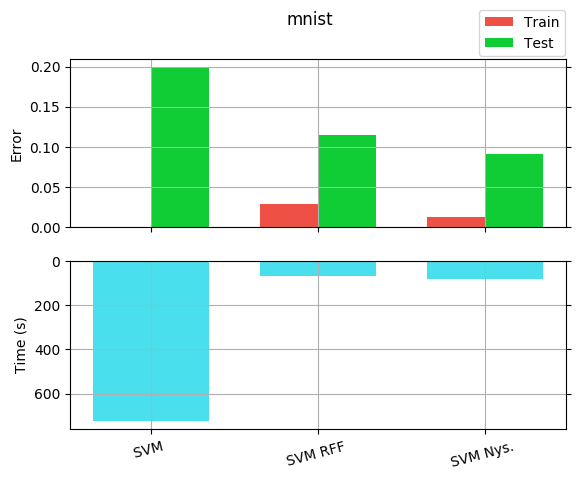
\includegraphics[width=\imgscale\linewidth]{Figures/\filePrefix/mnist}
%     \caption{Exp. 4.2 with MNIST. Random Forest outperforms Ensembles of Decision Tree with RFF.}
%     \label{fig:\undPrefix_mnist}
%   \end{subfigure}
% \end{figure}
%
%
% \begin{figure}[H]
%   \centering
%   \begin{subfigure}[t]{0.5\linewidth}
%     \centering\captionsetup{width=.8\linewidth}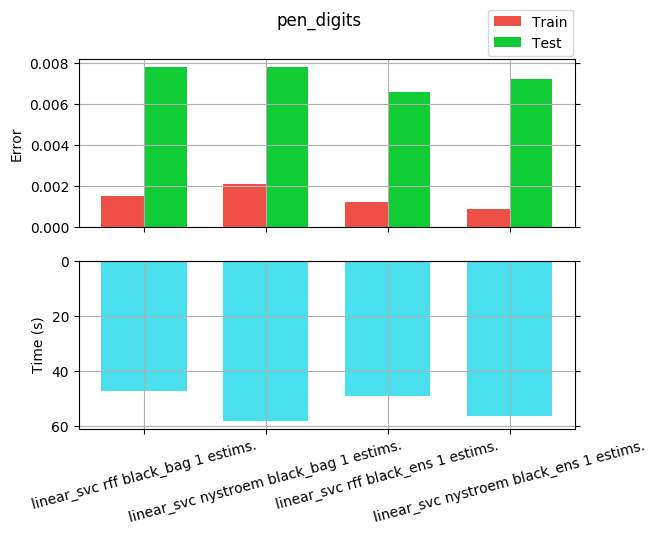
\includegraphics[width=\imgscale\linewidth]{Figures/\filePrefix/pen_digits}
%     \caption{Exp. 4.2 with Pen Digits. Random Forest outperforms Ensembles of Decision Tree with RFF.}
%     \label{fig:\undPrefix_pen_digits}
%   \end{subfigure}%
%   \begin{subfigure}[t]{0.5\linewidth}
%     \centering\captionsetup{width=.8\linewidth}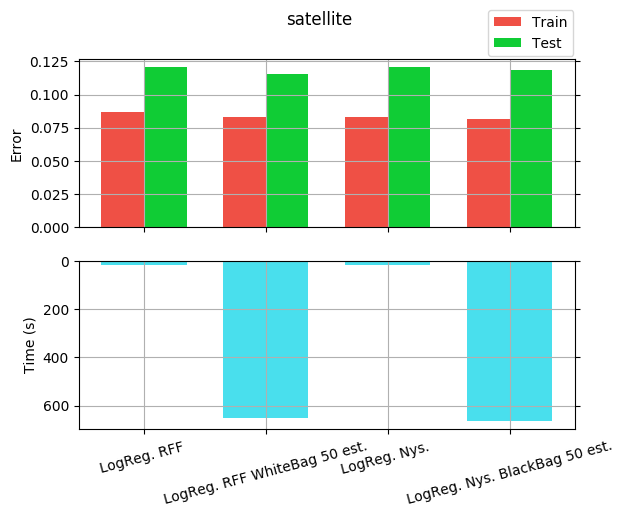
\includegraphics[width=\imgscale\linewidth]{Figures/\filePrefix/satellite}
%     \caption{Exp. 4.2 with Satellite. Random Forest outperforms Ensembles of Decision Tree with RFF.}
%     \label{fig:\undPrefix_satellite}
%   \end{subfigure}
% \end{figure}
%
% \begin{figure}[H]
%   \centering
%   \begin{subfigure}[t]{0.5\linewidth}
%     \centering\captionsetup{width=.8\linewidth}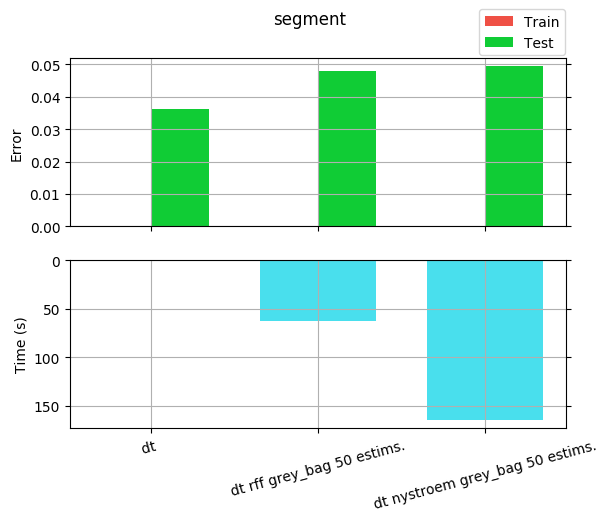
\includegraphics[width=\imgscale\linewidth]{Figures/\filePrefix/segment}
%     \caption{Exp. 4.2 with Segment. Random Forest outperforms Ensembles of Decision Tree with RFF.}
%     \label{fig:\undPrefix_segment}
%   \end{subfigure}%
%   \begin{subfigure}[t]{0.5\linewidth}
%     \centering\captionsetup{width=.8\linewidth}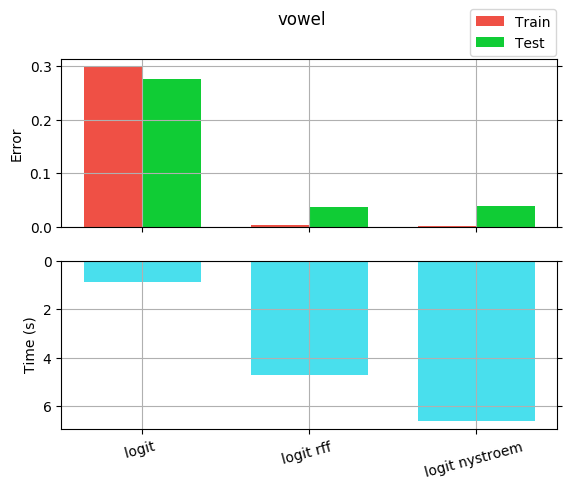
\includegraphics[width=\imgscale\linewidth]{Figures/\filePrefix/vowel}
%     \caption{Exp. 4.2 with Vowel. Random Forest outperforms Ensembles of Decision Tree with RFF.}
%     \label{fig:\undPrefix_vowel}
%   \end{subfigure}
% \end{figure}
%
% %%%%%%%%%%%%%%%%%%%%%%%%%%%%%%
%
% \renewcommand{\filePrefix}{\undPrefix/nys}
% \begin{figure}[H]
%   \centering
%   \begin{subfigure}[t]{0.5\linewidth}
%     \centering\captionsetup{width=.8\linewidth}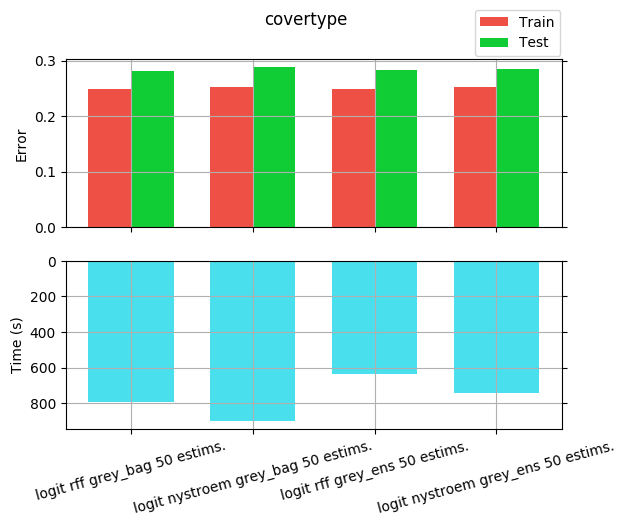
\includegraphics[width=\imgscale\linewidth]{Figures/\filePrefix/covertype}
%     \caption{Exp. 4.2 with Covertype. Random Forest outperforms Ensembles of Decision Tree with \Nys.}
%     \label{fig:\undPrefix_covertype}
%   \end{subfigure}%
%   \begin{subfigure}[t]{0.5\linewidth}
%     \centering\captionsetup{width=.8\linewidth}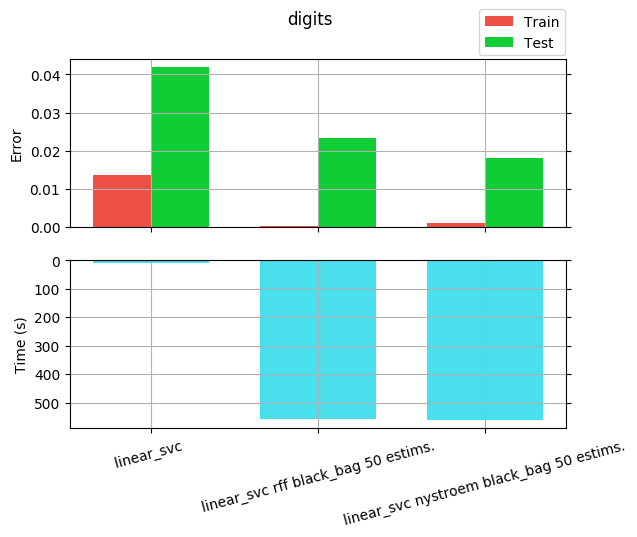
\includegraphics[width=\imgscale\linewidth]{Figures/\filePrefix/digits}
%     \caption{Exp. 4.2 with Digits. Random Forest outperforms Ensembles of Decision Tree with \Nys.}
%     \label{fig:\undPrefix_digits}
%   \end{subfigure}
% \end{figure}
%
%
% \begin{figure}[H]
%   \centering
%   \begin{subfigure}[t]{0.5\linewidth}
%     \centering\captionsetup{width=.8\linewidth}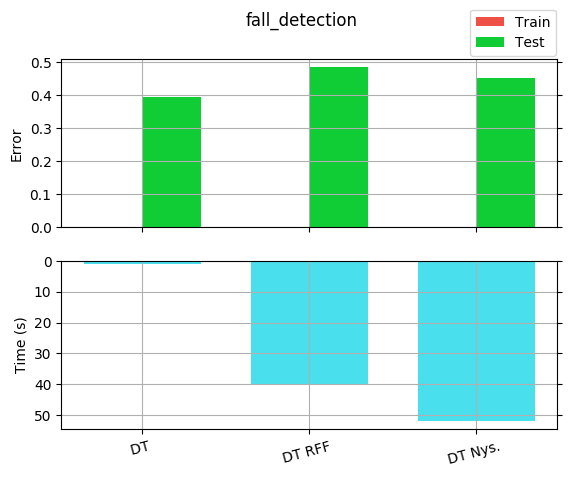
\includegraphics[width=\imgscale\linewidth]{Figures/\filePrefix/fall_detection}
%     \caption{Exp. 4.2 with Fall Detection. Random Forest outperforms Ensembles of Decision Tree with \Nys.}
%     \label{fig:\undPrefix_fall_detection}
%   \end{subfigure}%
%   \begin{subfigure}[t]{0.5\linewidth}
%     \centering\captionsetup{width=.8\linewidth}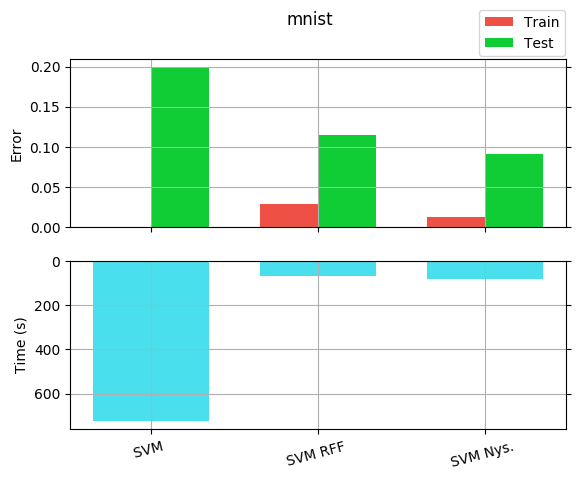
\includegraphics[width=\imgscale\linewidth]{Figures/\filePrefix/mnist}
%     \caption{Exp. 4.2 with MNIST. Random Forest outperforms Ensembles of Decision Tree with \Nys.}
%     \label{fig:\undPrefix_mnist}
%   \end{subfigure}
% \end{figure}
%
%
% \begin{figure}[H]
%   \centering
%   \begin{subfigure}[t]{0.5\linewidth}
%     \centering\captionsetup{width=.8\linewidth}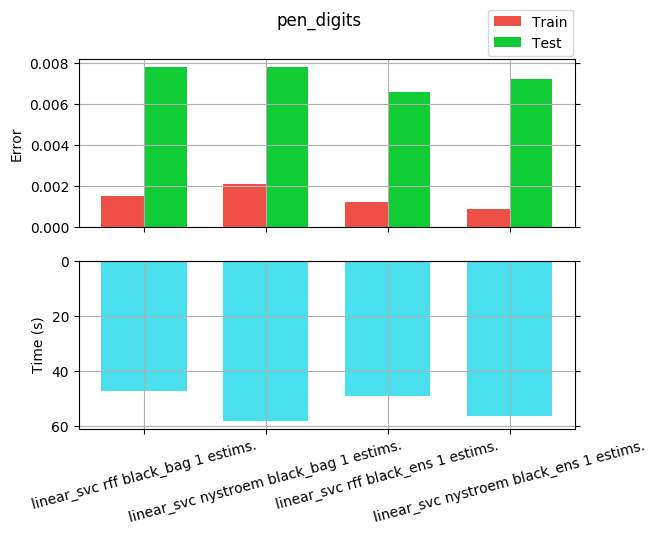
\includegraphics[width=\imgscale\linewidth]{Figures/\filePrefix/pen_digits}
%     \caption{Exp. 4.2 with Pen Digits. Random Forest outperforms Ensembles of Decision Tree with \Nys.}
%     \label{fig:\undPrefix_pen_digits}
%   \end{subfigure}%
%   \begin{subfigure}[t]{0.5\linewidth}
%     \centering\captionsetup{width=.8\linewidth}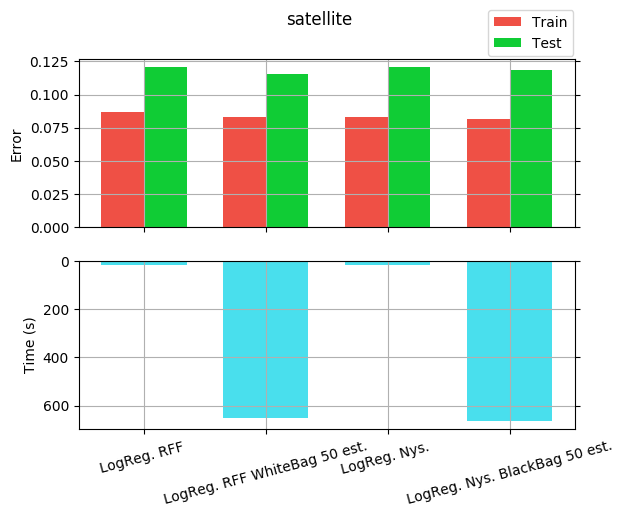
\includegraphics[width=\imgscale\linewidth]{Figures/\filePrefix/satellite}
%     \caption{Exp. 4.2 with Satellite. Random Forest outperforms Ensembles of Decision Tree with \Nys.}
%     \label{fig:\undPrefix_satellite}
%   \end{subfigure}
% \end{figure}
%
% \begin{figure}[H]
%   \centering
%   \begin{subfigure}[t]{0.5\linewidth}
%     \centering\captionsetup{width=.8\linewidth}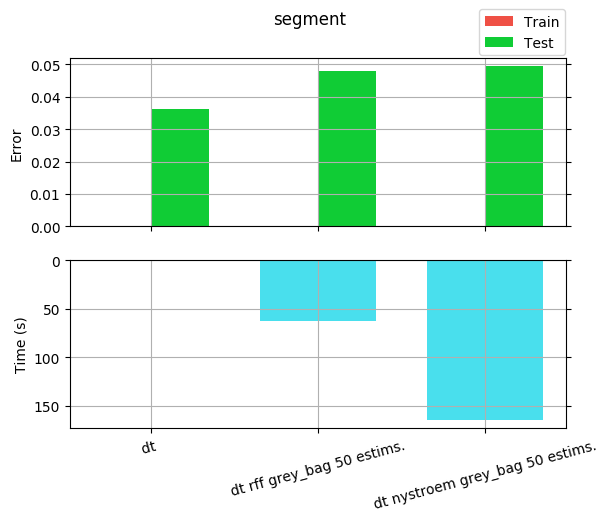
\includegraphics[width=\imgscale\linewidth]{Figures/\filePrefix/segment}
%     \caption{Exp. 4.2 with Segment. Random Forest outperforms Ensembles of Decision Tree with \Nys.}
%     \label{fig:\undPrefix_segment}
%   \end{subfigure}%
%   \begin{subfigure}[t]{0.5\linewidth}
%     \centering\captionsetup{width=.8\linewidth}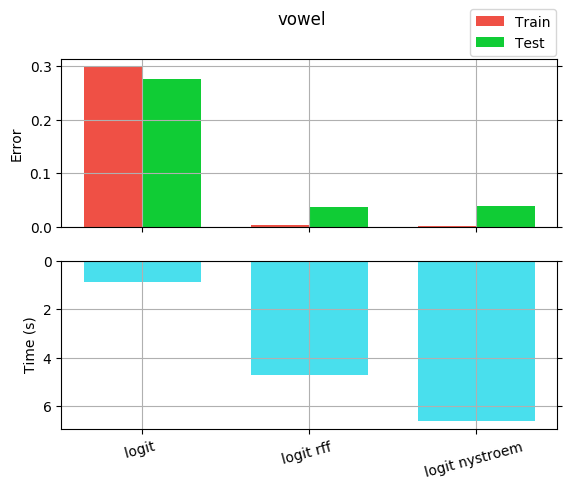
\includegraphics[width=\imgscale\linewidth]{Figures/\filePrefix/vowel}
%     \caption{Exp. 4.2 with Vowel. Random Forest outperforms Ensembles of Decision Tree with \Nys.}
%     \label{fig:\undPrefix_vowel}
%   \end{subfigure}
% \end{figure}


\let\major\undefined
\let\minor\undefined

\let\undPrefix\undefined
\let\dotPrefix\undefined
\let\scoPrefix\undefined

\let\filePrefix\undefined
